% !TEX TS-program = knitr
\documentclass{article}\usepackage{graphicx, color}
%% maxwidth is the original width if it is less than linewidth
%% otherwise use linewidth (to make sure the graphics do not exceed the margin)
\makeatletter
\def\maxwidth{ %
  \ifdim\Gin@nat@width>\linewidth
    \linewidth
  \else
    \Gin@nat@width
  \fi
}
\makeatother

\IfFileExists{upquote.sty}{\usepackage{upquote}}{}
\definecolor{fgcolor}{rgb}{0.2, 0.2, 0.2}
\newcommand{\hlnumber}[1]{\textcolor[rgb]{0,0,0}{#1}}%
\newcommand{\hlfunctioncall}[1]{\textcolor[rgb]{0.501960784313725,0,0.329411764705882}{\textbf{#1}}}%
\newcommand{\hlstring}[1]{\textcolor[rgb]{0.6,0.6,1}{#1}}%
\newcommand{\hlkeyword}[1]{\textcolor[rgb]{0,0,0}{\textbf{#1}}}%
\newcommand{\hlargument}[1]{\textcolor[rgb]{0.690196078431373,0.250980392156863,0.0196078431372549}{#1}}%
\newcommand{\hlcomment}[1]{\textcolor[rgb]{0.180392156862745,0.6,0.341176470588235}{#1}}%
\newcommand{\hlroxygencomment}[1]{\textcolor[rgb]{0.43921568627451,0.47843137254902,0.701960784313725}{#1}}%
\newcommand{\hlformalargs}[1]{\textcolor[rgb]{0.690196078431373,0.250980392156863,0.0196078431372549}{#1}}%
\newcommand{\hleqformalargs}[1]{\textcolor[rgb]{0.690196078431373,0.250980392156863,0.0196078431372549}{#1}}%
\newcommand{\hlassignement}[1]{\textcolor[rgb]{0,0,0}{\textbf{#1}}}%
\newcommand{\hlpackage}[1]{\textcolor[rgb]{0.588235294117647,0.709803921568627,0.145098039215686}{#1}}%
\newcommand{\hlslot}[1]{\textit{#1}}%
\newcommand{\hlsymbol}[1]{\textcolor[rgb]{0,0,0}{#1}}%
\newcommand{\hlprompt}[1]{\textcolor[rgb]{0.2,0.2,0.2}{#1}}%

\usepackage{framed}
\makeatletter
\newenvironment{kframe}{%
 \def\at@end@of@kframe{}%
 \ifinner\ifhmode%
  \def\at@end@of@kframe{\end{minipage}}%
  \begin{minipage}{\columnwidth}%
 \fi\fi%
 \def\FrameCommand##1{\hskip\@totalleftmargin \hskip-\fboxsep
 \colorbox{shadecolor}{##1}\hskip-\fboxsep
     % There is no \\@totalrightmargin, so:
     \hskip-\linewidth \hskip-\@totalleftmargin \hskip\columnwidth}%
 \MakeFramed {\advance\hsize-\width
   \@totalleftmargin\z@ \linewidth\hsize
   \@setminipage}}%
 {\par\unskip\endMakeFramed%
 \at@end@of@kframe}
\makeatother

\definecolor{shadecolor}{rgb}{.97, .97, .97}
\definecolor{messagecolor}{rgb}{0, 0, 0}
\definecolor{warningcolor}{rgb}{1, 0, 1}
\definecolor{errorcolor}{rgb}{1, 0, 0}
\newenvironment{knitrout}{}{} % an empty environment to be redefined in TeX

\usepackage{alltt}

\usepackage{amsfonts}
\usepackage{amsmath}
\usepackage{amssymb}
\usepackage{amsthm}
\usepackage{caption}
\usepackage{color}
\usepackage{enumerate}
\usepackage{fancyhdr}
\usepackage{hyperref}
\usepackage{graphicx}
\usepackage{latexsym}
\usepackage{listings}
\usepackage{mathrsfs}
\usepackage{natbib}
\usepackage[nottoc]{tocbibind}
\usepackage{url}

\providecommand{\all}{\ \forall \ }
\providecommand{\bs}{\backslash}
\providecommand{\e}{\varepsilon}
\providecommand{\E}{\ \exists \ }
\providecommand{\lm}[2]{\lim_{#1 \rightarrow #2}}
\providecommand{\m}[1]{\mathbb{#1}}
\providecommand{\nv}{{}^{-1}}
\providecommand{\ov}[1]{\overline{#1}}
\providecommand{\p}{\newpage}
\providecommand{\q}{$\quad$ \newline}
\providecommand{\rt}{\rightarrow}
\providecommand{\Rt}{\Rightarrow}
\providecommand{\vc}[1]{\boldsymbol{#1}}
\providecommand{\wh}[1]{\widehat{#1}}

%\renewcommand\bibname{References}
%\renewcommand{\thesection}{Problem \arabic{section}}
%\renewcommand{\thesubsection}{Part \alph{subsection}}
\numberwithin{equation}{section}

\fancyhead{}
\fancyfoot{}
\fancyhead[R]{\thepage}
\fancyhead[C]{Landau}

\hypersetup{
    colorlinks,
    citecolor=black,
    filecolor=black,
    linkcolor=black,
    urlcolor=blue
}

\definecolor{dkgreen}{rgb}{0,0.6,0}
\definecolor{gray}{rgb}{0.5,0.5,0.5}
\definecolor{mauve}{rgb}{0.58,0,0.82}

\lstset{ 
  language=C,                % the language of the code
  basicstyle=\Large,           % the size of the fonts that are used for the code
  numberstyle= \tiny \color{white},  % the style that is used for the line-numbers
  stepnumber=2,                   % the step between two line-numbers. 
  numbersep=5pt,                  % how far the line-numbers are from the code
  backgroundcolor=\color{white},      % choose the background color. You must add \usepackage{color}
  showspaces=false,               % show spaces adding particular underscores
  showstringspaces=false,         % underline spaces within strings
  showtabs=false,                 % show tabs within strings adding particular underscores
  frame=lrb,                   % adds a frame around the code
  rulecolor=\color{black},        % if not set, the frame-color may be changed on line-breaks within not-black text 
  tabsize=2,                      % sets default tabsize to 2 spaces
  captionpos=t,                   % sets the caption-position 
  breaklines=true,                % sets automatic line breaking
  breakatwhitespace=false,        % sets if automatic breaks should only happen at whitespace
  title=\lstname,                   % show the filename of files included with \lstinputlisting;
  keywordstyle=\color{blue},          % keyword style
  commentstyle=\color{gray},       % comment style
  stringstyle=\color{dkgreen},         % string literal style
  escapeinside={\%*}{*)},            % if you want to add LaTeX within your code
  morekeywords={*, ...},               % if you want to add more keywords to the set
  xleftmargin=0.053in, % left horizontal offset of caption box
  xrightmargin=-.03in % right horizontal offset of caption box
}

\DeclareCaptionFont{white}{\color{white}}
\DeclareCaptionFormat{listing}{\parbox{\textwidth}{\colorbox{gray}{\parbox{\textwidth}{#1#2#3}}\vskip-0.05in}}
\captionsetup[lstlisting]{format = listing, labelfont = white, textfont = white}
% For caption-free listings, comment out the 3 lines above and uncomment the 2 lines below.
% \captionsetup{labelformat = empty, labelsep = none}
% \lstset{frame = single}






\begin{document}



\begin{flushleft}


\begin{center} \LARGE
STAT 305 D Homework 1 Solutions
\end{center}
\begin{center} \Large
Due January 24, 2012 at 12:40 PM in class
\end{center}

{\Large
\color{blue} EXTRA CREDIT: complete the survey at http://www.surveymonkey.com/s/M7WK3PG before you hand in this assignment.}



\begin{enumerate}[1. ]
 \setcounter{enumi}{0}

\item Vardeman and Jobe Chapter 1 Section 2 Exercise 1 (page 13):

\setkeys{Gin}{width=.5\textwidth} 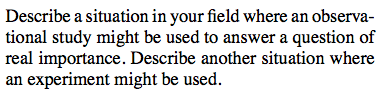
\includegraphics{../../fig/ch1s2p1.png}
\setkeys{Gin}{width=1\textwidth} 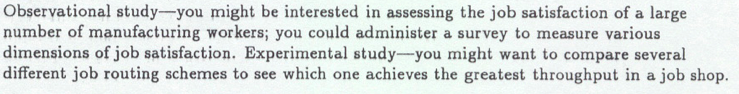
\includegraphics{../../fig/ch1s2p1sol.png}

\item Vardeman and Jobe Chapter 1 Section 2 Exercise 2 (page 13):

\setkeys{Gin}{width=.5\textwidth} 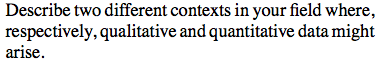
\includegraphics{../../fig/ch1s2p2.png}
\setkeys{Gin}{width=1\textwidth} 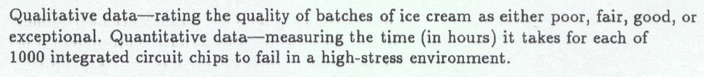
\includegraphics{../../fig/ch1s2p2sol.png}

\item Vardeman and Jobe Chapter 1 Section 2 Exercise 6 (page 14):

\setkeys{Gin}{width=.5\textwidth} 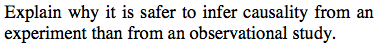
\includegraphics{../../fig/ch1s2p6.png}
\setkeys{Gin}{width=1\textwidth} 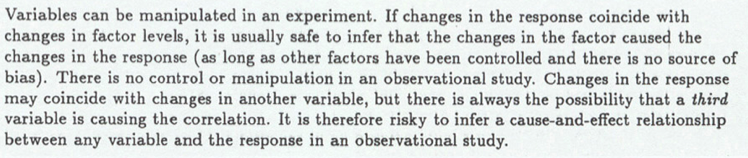
\includegraphics{../../fig/ch1s2p6sol.png}

In addition, the randomization of sample units to treatment groups ensures that the treatment variable is uncorrelated with all experimental conditions, which is another condition necessary for deducing causality.

\item Vardeman and Jobe Chapter 1 Section 3 Exercise 1 (page 19):

\setkeys{Gin}{width=.5\textwidth} 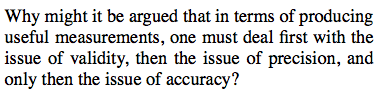
\includegraphics{../../fig/ch1s3p1.png}
\setkeys{Gin}{width=1\textwidth} 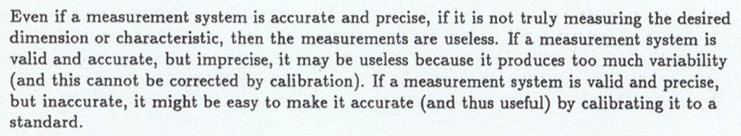
\includegraphics{../../fig/ch1s3p1sol.png} 

\item Vardeman and Jobe Chapter 1 Section 3 Exercise 2 (page 19): Often, in order to evaluate a physical quantity (for example, the mean yield of a batch chemical process run according to some standard plant operating procedures), a large number of measurements of the quantity are made and then averaged. (The alternative is just to use an individual measurement in place of an average.) Explain which of the three aspects of measurement quality - validity, precision, and accuracy - this averaging of many measurements can be expected to improve and which it cannot.

\setkeys{Gin}{width=1\textwidth} 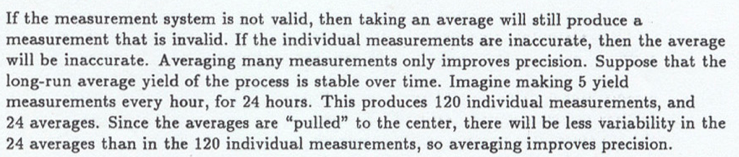
\includegraphics{../../fig/ch1s3p2sol.png}

\item  A group of chemists and chemical engineers tested their newly-designed Type I Diabetes medication on rats. The goal was to figure out if the medicine would improve the conditions of Type I Diabetes-afflicted rats in general (future work will be on humans). 18 rats with Type I diabetes were randomly selected for the study. Half of these 18 rats were randomly selected to be given the medicine, and the others were not given any medicine. For each rat, the investigators recorded the improvement of of the rat's physical fitness over the duration of the experiment (measured according to initial and final stress tests). The weight of each rat on the first day of the study was passively recorded. The investigators made sure that the distribution of food, room temperature, opportunity for exercise, etc., was the same for each rat for the duration of the study.

\begin{enumerate}[a. ]
\item What is the population of interest for this study? What is the sample? 

\begin{itemize}
\item {\color{red} Population: All Type I Diabetes-afflicted rats. }
\item {\color{red} Sample: the 18 diabetes-afflicted in the study.}
\end{itemize}


\item Is this study an experiment or an observational study? Why? \q

{\color{red} Experiment: the investigators applied the medication (treatment) themselves while keeping experimental conditions constant for each rat (and thus for each level of treatment).} \q

\item Identify and classify all the variables in this study.

{\color{red}
\begin{itemize}
\item Treatment: medication level
\item Response: improvement in rat fitness 
\end{itemize}}

\item Identify the treatment groups, if any, and state how many there are. \q

{\color{red} There are 2 experimental groups: one with the rats who were given the medication, one with the rats who were not given the medication. }

\end{enumerate} \q

\item Weekly feedback. You get full credit as long as you write something.
\begin{enumerate}[1. ]
\item Is there any aspect of the subject matter that you currently struggle with? If so, what specifically do you find difficult or confusing? The more detailed you are, the better I can help you.
{\color{red} You got full credit as long as you wrote something.}
\item Do you have any questions or concerns about the material, class logistics, or anything else? If so, fire away.
{\color{red} You got full credit as long as you wrote something.}
\end{enumerate}

\end{enumerate}




\end{flushleft}
%\newpage 
%\nocite{*}
%\bibliographystyle{plainnat} 
%\bibliography{}
\end{document}
